% !TeX spellcheck = it_IT

\documentclass[xcolor={x11names}]{beamer}
\usetheme{Berkeley}
\setbeamercolor*{structure}{bg=DodgerBlue3!20,fg=DodgerBlue3}
\setbeamercolor*{sidebar}{use=structure,bg=structure.fg!68!black}
\setbeamercolor*{palette primary}{use=structure,fg=white,bg=structure.fg}
\setbeamercolor*{palette secondary}{use=structure,fg=white,bg=structure.fg!70}
\setbeamercolor*{palette tertiary}{use=structure,fg=white,bg=structure.fg!50!black}
\setbeamercolor*{palette quaternary}{fg=white,bg=black}
\setbeamercolor*{alerted text}{use=structure,fg={structure.fg>wheel,2,5}}
\usefonttheme{serif}
%\usefonttheme{structuresmallcapsserif} %forse un po' troppo pretenzioso

\usepackage[english,italian]{babel}
\usepackage{siunitx}
\usepackage{tikz}
\usepackage{pgfplots}
\usepackage{pgfplotstable}
\pgfplotsset{
	compat=newest,
	every tick label/.append style={font=\tiny},
	every node near coord/.append style={font=\scriptsize,color=black},
	label style={font=\small},
	legend style={font=\small}
}
\usepgfplotslibrary{ternary}
\usetikzlibrary{calc}
\usepackage{url}
\usepackage[export]{adjustbox}
\usepackage[font={footnotesize,color=darkgray},justification=centering]{caption}
\usepackage{calc}

\title{OpenLDAT}
\subtitle{Un sistema di misurazione di metriche di latenza dei display}
\author{Federico Dossena}
\date{Anno Accademico 2020/2021}

\newlength\leftsidebar
\newlength\rightsidebar
\makeatletter
\setlength\leftsidebar{\beamer@leftsidebar}
\setlength\rightsidebar{\beamer@rightsidebar}
\makeatother

\begin{document}

\setbeamertemplate{navigation symbols}{} %rimuovi i bottoni di navigazione in basso
\hoffset=-1\leftsidebar %rimuovi il bordo a sx per la sidebar
\begin{frame}[plain]
	\begin{minipage}{\textwidth+1\leftsidebar}
		\begin{center}
			
\includegraphics[width=0.6\textwidth]{Logo.png}\\
			\usebeamerfont{institute}{\bf Corso di Laurea Magistrale in Informatica}
		\end{center}
		\begin{beamercolorbox}[sep=12pt,center]{title}
			\usebeamerfont{title} \inserttitle\\
			\vspace{1mm}
			\usebeamerfont{subtitle} \insertsubtitle
		\end{beamercolorbox}
		\begin{center}
			\begin{minipage}[t]{0.45\textwidth}
				\begin{flushleft}
					\usebeamerfont{institute}
					{\bf Relatore:}\\
					Prof. Andrea TRENTINI\\
					\vspace{2mm}
					{\bf Correlatore:}\\
					Prof. Alessandro RIZZI
				\end{flushleft}
			\end{minipage}
			\begin{minipage}[t]{0.45\textwidth}
				\begin{flushright}
					\usebeamerfont{institute}
					{\bf Tesi di Laurea di:}\\
					Federico DOSSENA\\
					Matr. 909390
				\end{flushright}
			\end{minipage}
		\end{center}
		\vspace{3mm}
		\begin{center}
			\usebeamerfont{institute} \insertdate
		\end{center}
	\end{minipage}
\end{frame}

\setbeamertemplate{navigation symbols}{ %ripristina i pulsanti di navigazione in basso
	\hbox{
		\hbox{\insertslidenavigationsymbol}
		\hbox{\insertframenavigationsymbol}
		\hbox{\insertsubsectionnavigationsymbol}
		\hbox{\insertsectionnavigationsymbol}
		\hbox{\insertdocnavigationsymbol}
		\hbox{\insertbackfindforwardnavigationsymbol}
	}
}
\hoffset=0mm %ripristina il bordo a sx per la sidebar

\section{Introduzione}
\begin{frame}
	\frametitle{Introduzione}
	\begin{itemize}
		\item Progetto nato dall'esigenza di \alert{misurare la latenza totale di un sistema}
		\item \alert{OpenLDAT può misurarla in modo automatico}, e può fare anche molto altro
		\item \alert{Nessun dispositivo simile sul mercato}, solitamente si usa un mouse con collegato un LED e una telecamera ad alta velocità
		\item Progetto totalmente \alert{libero}
	\end{itemize}
	\begin{block}{Latenza totale del sistema}
		Tempo che intercorre tra un'azione nel mondo fisico, come un click del mouse, e la visualizzazione del risultato sul display.
	\end{block}
\end{frame}

\section{Dispositivo}
\begin{frame}[shrink=10]
	\frametitle{Dispositivo OpenLDAT (1)}
	\begin{columns}
		\column{0.5\textwidth}
		\begin{itemize}
			\item Microcontroller \alert{ATmega32U4}
			\item Fototransistor \alert{ALS-PT19} con \alert{4 livelli di gain} del sensore controllabili via software
		\end{itemize}
		\column{0.5\textwidth}
		\begin{itemize}
			\item \alert{PCB} personalizzato
			\item Campionamento fino a \alert{\textasciitilde 30kHz 10-bit}
			\item Comunicazione via USB HID e CDC Serial, \alert{nessun driver richiesto}
		\end{itemize}
	\end{columns}
	\begin{figure}
		\centering
		\adjincludegraphics[trim={{.10\width} 0 {.20\width} 0},clip,height=0.55\textheight]{Dispositivo_files/assembly_10.jpg}
		\adjincludegraphics[trim={{.12\width} 0 {.18\width} 0},clip,height=0.55\textheight]{Dispositivo_files/assembly_09.jpg}
		\caption*{Hardware del dispositivo OpenLDAT}
	\end{figure}
\end{frame}
\begin{frame}
	\frametitle{Dispositivo OpenLDAT (2)}
	\begin{columns}
		\column{0.5\textwidth}
		\begin{itemize}
			\item Generazione dei \alert{click automatica o manuale} tramite input esterno
			\item \alert{LED per validazione} con telecamera ad alta velocità
			\item \alert{Case stampabile} in 3D
			\item \alert{Poco costoso e facile da realizzare} anche da un maker
		\end{itemize}
		\column{0.5\textwidth}
		\begin{figure}
			\adjincludegraphics[trim={{.22\width} 0 {.22\width} 0},clip,width=\textwidth]{Dispositivo_files/assembly_15.jpg}
			\caption*{Dispositivo OpenLDAT assemblato}
		\end{figure}
	\end{columns}
\end{frame}

\section{Applicazione}
\begin{frame}[shrink=15]
	\frametitle{Applicazione OpenLDAT (1)}
	\begin{columns}
		\column{0.5\textwidth}
		\begin{itemize}
			\item \alert{Applicazione grafica} Java SE e OpenGL
			\item Permette di \alert{configurare ed eseguire i test, e visualizzarne i risultati} in modo semplice
		\end{itemize}
		\column{0.5\textwidth}
		\begin{itemize}
			\item \alert{Esportazione dei dati} per analisi esterna
			\item \alert{Include un manuale} dei test
			\item \alert{Multipiattaforma} (Windows, GNU/Linux, MacOS)
		\end{itemize}
	\end{columns}
	\begin{figure}
		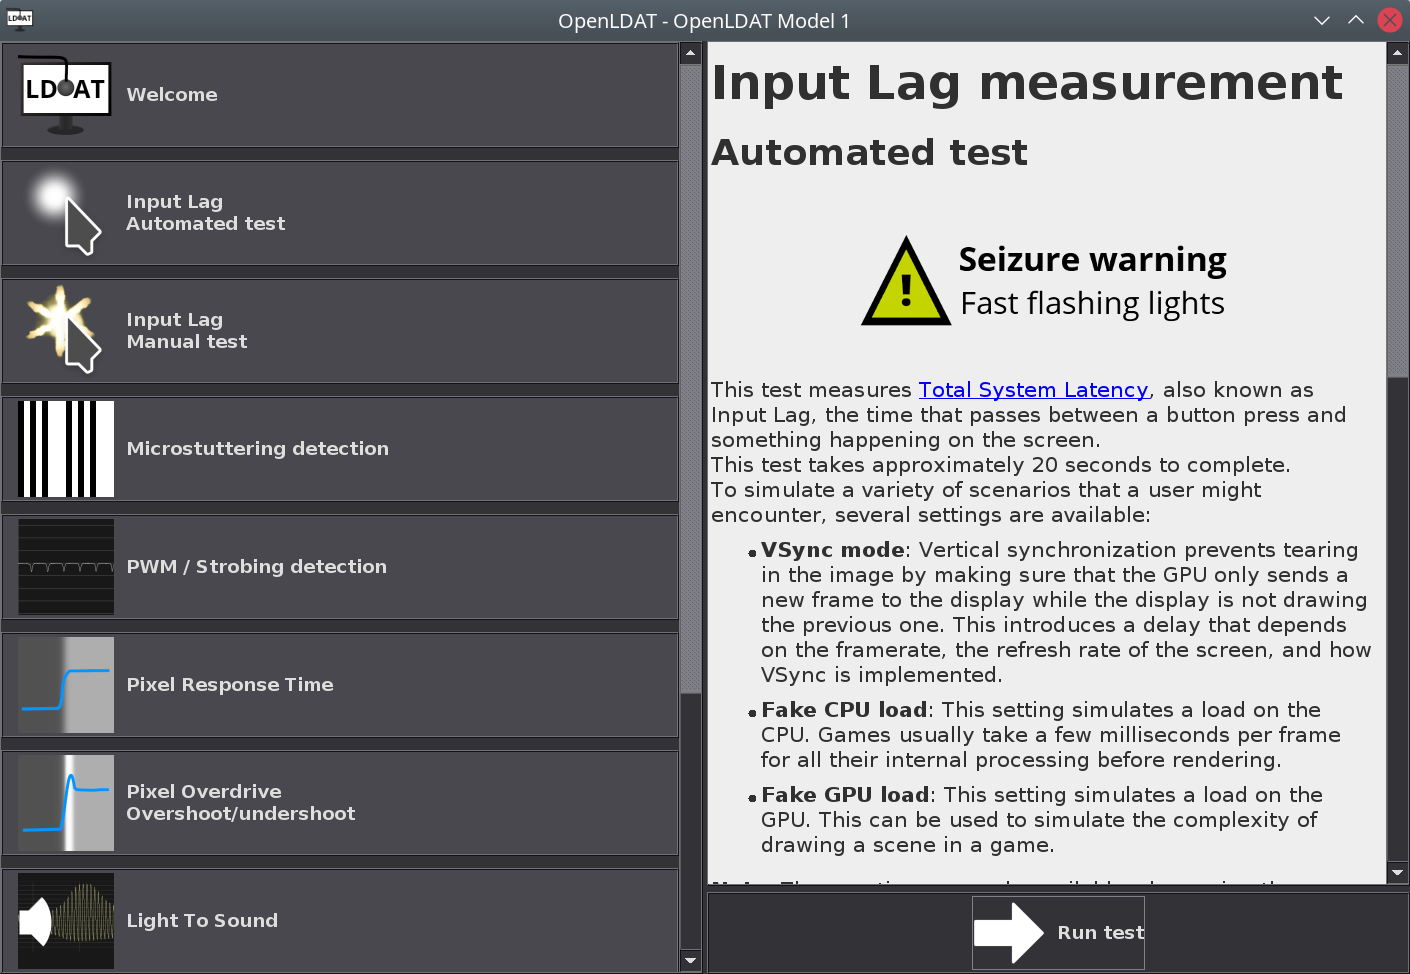
\includegraphics[height=0.7\textheight]{Applicazione_files/gui_mainMenu2.png}
		\caption*{Schermata principale dell'applicazione}
	\end{figure}
\end{frame}
\begin{frame}[shrink=3]
	\frametitle{Applicazione OpenLDAT (2)}
	\begin{itemize}
		\item \alert{Latenza totale del sistema}:\begin{itemize}
			\item \alert{Test automatico} con OpenGL e generazione automatica dei click
			\item \alert{Test interattivo} utilizzando un'applicazione e la generazione automatica dei click o un mouse/controller modificato
		\end{itemize}
		\item \alert{Rilevamento del microstuttering}: rileva perdita/duplicazione di fotogrammi
		\item \alert{Rilevamento di PWM e noise}: rileva la frequenza del lampeggio della retroilluminazione e altri tipi di rumore
		\item \alert{Tempi di risposta dei pixel}: misura il tempo di transizione dei pixel
		\item \alert{Overdrive dei pixel}: misura l'errore commesso durante la transizione dei pixel
		\item \alert{Light to Sound}: permette di ascoltare il segnale dal sensore, utile per rilevare fonti di rumore
	\end{itemize}
\end{frame}
\begin{frame}[shrink=10]
	\frametitle{Applicazione OpenLDAT (3)}
	\begin{figure}
		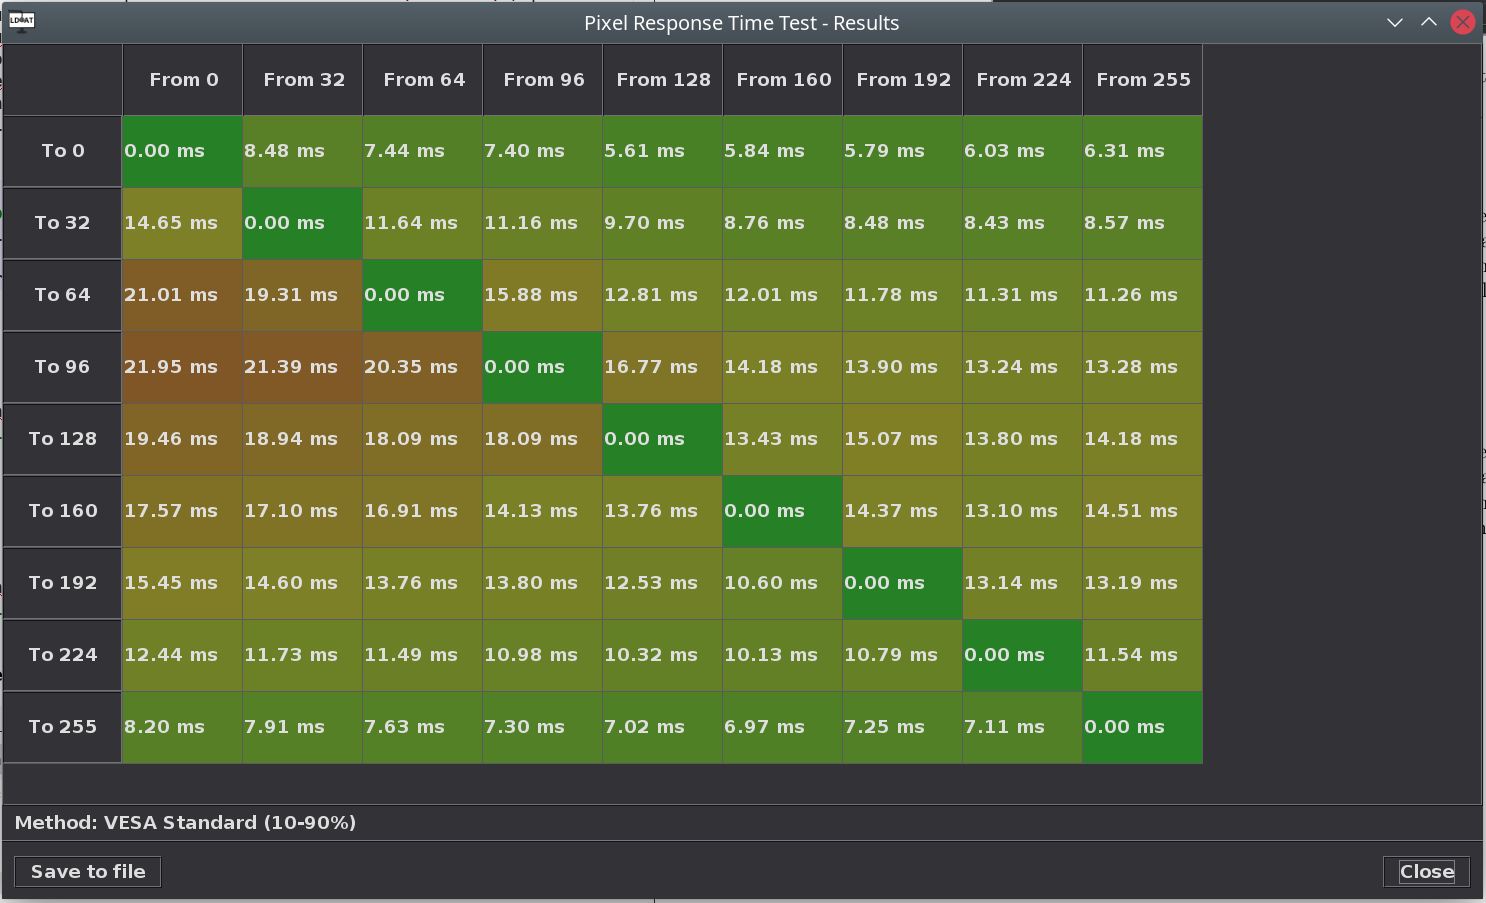
\includegraphics[width=\textwidth]{Applicazione_files/gui_pixelresponse_results.png}
		\caption*{Esempio di risultati di un test dei tempi di risposta dei pixel (AOC Q2770P)}
	\end{figure}
\end{frame}

\section{Risultati sperimentali}
\begin{frame}
	\frametitle{Risultati sperimentali}
	\begin{itemize}
		\item Sono stati testati \alert{oltre 20 display di tipi e periodi diversi} con modalità controllate
		\item Test eseguiti anche su \alert{combinazioni hardware e software diverse} per determinarne l'impatto
		\item Oltre ai test automatici, sono anche state \alert{testate diverse applicazioni} per determinare quanto l'implementazione impatti le prestazioni
		\item In fase di test sono emersi \alert{alcuni comportamenti interessanti}
		\item Sono stati selezionati alcuni test rappresentativi per questa presentazione
	\end{itemize}
\end{frame}
\begin{frame}[fragile,shrink=20]
	\frametitle{Input lag (1)}
	\begin{columns}
		\column{0.35\textwidth}
		\begin{itemize}
			\setlength\itemsep{1mm}
			\item I display ad \alert{alto refresh rate hanno il ritardo minore}
			\item Alcuni display hanno un ritardo inferiore a un refresh, quindi \alert{mostrano l'immagine mentre la stanno ricevendo}
			\item Altri aspettano di avere 1+ fotogrammi prima di visualizzarli per \alert{applicare dell'elaborazione}
			\item I \alert{televisori hanno il ritardo peggiore}
		\end{itemize}
		\column{0.65\textwidth}
		\begin{figure}
			\pgfplotstableread[col sep=comma]{
				model,novsync,vsync
				Acer Predator XB271HU (165Hz G-Sync),6.3,32.5
				Samsung C34H890 (100Hz Freesync),11.8,52.8
				ASUS VP228HE (60Hz),13.1,86.8
				LG E2360 (60Hz),14.1,89.6
				BenQ GL2706PQ (60Hz),27.7,93.7
				AOC Q2770P (60Hz),29.8,95.8
				Sharp LC-40FG3242E (60Hz TV),37.1,108.8
				Samsung P2770HD (60Hz TV),41.1,111.9
			}\dataset
			\begin{tikzpicture}
				\begin{axis}[xbar, bar width=8pt, y dir=reverse, ytick=data, yticklabels from table={\dataset}{model}, yticklabel style={text width=2.5cm, align=right}, table/y expr = \coordindex, nodes near coords, reverse legend, legend style={at={(5.25cm,-0.75cm)},anchor=east},xlabel=Ritardo (ms), width=6.5cm, height=8.25cm, xmin=0, ymin=-1, ymax=8, axis x line*=bottom, axis y line*=left] %ymax messo a mano con il numero di display per migliore formattazione
					\addplot table[x=vsync] {\dataset};
					\addplot table[x=novsync] {\dataset};
					\legend{VSync On, VSync Off}
				\end{axis}
			\end{tikzpicture}
			\caption*{Input lag di alcuni dei display testati}
		\end{figure}
	\end{columns}
\end{frame}
\begin{frame}[fragile,shrink=20]
	\frametitle{Input lag (2)}
	\begin{columns}
		\column{0.35\textwidth}
		\begin{itemize}
			\setlength\itemsep{1mm}
			\item Il \alert{driver Nvidia per Linux ha dato i risultati migliori}, nonostante la pessima reputazione
			\item Il \alert{ritardo su Linux è leggermente inferiore rispetto a Windows}, almeno per OpenGL
			\item Le \alert{GPU Intel hanno un ritardo maggiore}, probabilmente a causa del framerate inferiore durante il test
		\end{itemize}
		\column{0.65\textwidth}
		\begin{figure}
			\pgfplotstableread[col sep=comma]{
				config,novsync,vsync
				Linux Nvidia,28.0,69.1
				Windows Nvidia,28.4,95.3
				Linux AMD,28.7,86.1
				Windows AMD,29.6,93.9
				Windows Intel,31.3,103.4
				Linux Intel,34.1,86.6
				Linux Nouveau,44.3,86.0
			}\dataset
			\begin{tikzpicture}
				\begin{axis}[xbar, bar width=8pt, y dir=reverse, ytick=data, yticklabels from table={\dataset}{config}, yticklabel style={text width=1cm, align=right}, table/y expr = \coordindex, nodes near coords, reverse legend, legend style={at={(0.5,5.8cm)},anchor=south}, xlabel=Ritardo (ms), width=7cm, height=7.5cm, ymin=-1, ymax=7,xmax=110, axis x line*=bottom, axis y line*=left]
					\addplot table[x=vsync] {\dataset};
					\addplot table[x=novsync] {\dataset};
					\legend{VSync On, VSync Off}
				\end{axis}
			\end{tikzpicture}
			\caption*{Input lag con combinazioni hardware/software diverse}
		\end{figure}
	\end{columns}
\end{frame}
\begin{frame}[fragile,shrink=12]
	\frametitle{Input lag (3)}
	\begin{columns}
		\column{0.35\textwidth}
		\begin{itemize}
			\setlength\itemsep{1mm}
			\item Utilizzato il \alert{test manuale} su alcune applicazioni
			\item \alert{150ms è generalmente considerato il limite accettabile} per un videogioco, 400ms per un'applicazione
			\item \alert{Ritardo di Google Stadia diminuito rispetto al lancio} (era 180-300ms), ma varianza molto elevata
		\end{itemize}
		\column{0.65\textwidth}
		\begin{figure}
			\pgfplotstableread[col sep=comma]{
				app,lag,emin,emax
				Mass Effect Legendary Ed. (2021),45.7,8.4,7.7
				Crysis (2007),51.9,6.7,8.6
				Doom Eternal (2020),52.8,4.6,2.4
				Unreal Tournament 2004 (2003),81.3,11.8,18.7
				Google Stadia 1080p60 (FTTH),121.4,34.4,119.6
				YouTube (Chromium),147.2,13.0,17.2
				Doom (1993),158.9,16.9,14.2
				Crysis Remastered (2020),182.5,17.8,23.5
			}\dataset
			\begin{tikzpicture}
				\begin{axis}[xbar, bar width=10pt, y dir=reverse, ytick=data, yticklabels from table={\dataset}{app}, yticklabel style={text width=2cm, align=right}, table/y expr = \coordindex, nodes near coords, xlabel=Ritardo (ms), width=6.5cm, height=7.5cm, ymin=-1, ymax=8, axis x line*=bottom, axis y line*=left] %ymax messo a mano con il numero di test per migliore formattazione
					\addplot[fill=gray, error bars/.cd, x dir = both, x explicit] table[x=lag, x error plus=emax, x error minus=emin] {\dataset};
				\end{axis}
			\end{tikzpicture}
			\caption*{Input lag di alcune applicazioni}
		\end{figure}
	\end{columns}
\end{frame}
\begin{frame}[fragile,shrink=20]
	\frametitle{Tempi di risposta dei pixel e overdrive}
	\begin{itemize}
		\setlength\itemsep{1mm}
		\item Grafici mostrano \alert{media geometrica e varianza}
		\item Display recenti, TN, e "da gaming" hanno i migliori tempi di risposta
		\item Display \alert{IPS moderni non sono molto più lenti} rispetto ai TN
		\item \alert{Produttori spingono l'overdrive} per ridurre i tempi di risposta a scapito della qualità dell'immagine
	\end{itemize}
	
	\begin{minipage}{0.57\textwidth}
		\begin{figure}
			\centering
			\pgfplotstableread[col sep=comma]{
				model,odoff,odoffemin,odoffemax,odon,odonemin,odonemax,fix
				BenQ XL2420T (TN),NaN,NaN,NaN,2.61,1.48,3.80,-10
				Samsung C34H890 (VA),7.81,5.17,27.90,7.79,4.26,18.25,-10
				LG 27GL850-B (IPS HDR),9.74,3.94,4.46,2.91,1.92,11.69,-10
				AOC Q2770P (IPS),12.33,6.06,9.01,7.37,3.09,3.74,-10
				Octigen M19W (TN),14.61,13.10,13.03,NaN,NaN,NaN,-10
				MacBook Pro 13" 2017 (IPS),19.49,8.74,12.60,NaN,NaN,NaN,-10
			}\dataset
			\begin{tikzpicture}
				\begin{axis}[xbar, bar width=8pt, y dir=reverse, ytick=data, yticklabels from table={\dataset}{model}, yticklabel style={text width=2cm, align=right}, table/y expr = \coordindex, nodes near coords, reverse legend, xlabel=Tempo di risposta (ms), width=6.25cm, height=7cm, xmin=0, ymin=-1, ymax=6, axis x line*=bottom, axis y line*=left] %ymax messo a mano con il numero di display per migliore formattazione
					\addplot plot[forget plot] table[x=fix] {\dataset};
					\addplot plot [error bars/.cd, x dir = both, x explicit] table[x=odoff, x error plus=odoffemax, x error minus=odoffemin] {\dataset};
					\addplot plot [error bars/.cd, x dir = both, x explicit] table[x=odon, x error plus=odonemax, x error minus=odonemin] {\dataset};
					%\legend{Overdrive Off, Overdrive On}
				\end{axis}
			\end{tikzpicture}
			%\caption*{Tempi di riposta di alcuni dei display testati}
		\end{figure}
	\end{minipage}
	\begin{minipage}{0.33\textwidth}
		\begin{figure}
			\centering
			\pgfplotstableread[col sep=comma]{
				model,odoff,odoffemin,odoffemax,odon,odonemin,odonemax,fix
				,NaN,NaN,NaN,2.80,2.56,14.55,-10
				,0.32,0.32,1.79,1.21,1.21,6.43,-10
				,0.39,0.39,0.22,26.39,24.82,22.98,-10
				,0.17,0.17,0.41,4.14,4.14,16.32,-10
				,0.25,0.25,0.65,NaN,NaN,NaN,-10
				,0.22,0.22,0.59,NaN,NaN,NaN,-10
			}\dataset
			\begin{tikzpicture}
				\begin{axis}[xbar, bar width=8pt, y dir=reverse, ytick=data, yticklabels from table={\dataset}{model}, yticklabel style={text width=0cm, align=right}, table/y expr = \coordindex, nodes near coords, reverse legend, xlabel=Errore di transizione (\%), width=6.25cm, height=7cm, xmin=0, ymin=-1, ymax=6, axis x line*=bottom, axis y line*=left, legend style={at={(5.75cm,-0.75cm)},anchor=east}] %ymax messo a mano con il numero di display per migliore formattazione]
					\addplot plot[forget plot] table[x=fix] {\dataset};
					\addplot plot [error bars/.cd, x dir = both, x explicit] table[x=odoff, x error plus=odoffemax, x error minus=odoffemin] {\dataset};
					\addplot plot [error bars/.cd, x dir = both, x explicit] table[x=odon, x error plus=odonemax, x error minus=odonemin] {\dataset};
					\legend{Overdrive Off, Overdrive On}
				\end{axis}
			\end{tikzpicture}
			%\caption*{Errore di transizione in percentuale assoluta}
		\end{figure}
	\end{minipage}
\end{frame}
\begin{frame}
	\frametitle{Altri test}
	\begin{itemize}
		\setlength\itemsep{4mm}
		\item PWM e noise: \begin{itemize}
			\item \alert{Retroilluminazione PWM trovata solo su TV e display di fascia bassa}, tipicamente a 240Hz
			\item Nessuno dei display testati ha mostrato rumore sulla retroilluminazione
			\item \alert{Su alcuni display è rilevabile il ciclo di refresh dei pixel}
		\end{itemize}
		\item Microstuttering: \begin{itemize}
			\item \alert{Nessun display ha mostrato microstuttering a refresh rate nativo}
			\item \alert{Alcuni dei display hanno mostrato microstuttering in overclock}, ma non quelli "da gaming" o con refresh rate variabile
		\end{itemize}
	\end{itemize}
\end{frame}

\section{Conclusioni}
\begin{frame}
	\frametitle{Conclusioni}
	Durante lo sviluppo e il testing sono emersi diverse aree di miglioramento per le future iterazioni
	\begin{itemize}
		\item Aggiungere un \alert{colorimetro} per eseguire anche test sull'accuratezza dei colori
		\item Utilizzare un \alert{ADC con più bit} di precisione, per ridurre i livelli di gain necessari e permettere una misurazione accurata di livelli molto bassi di luminosità
		\item Aggiungere \alert{altri backend grafici e modalità di fullscreen} nell'applicazione, e \alert{migliorarne il supporto HDR}
		\item \alert{Portare l'applicazione} su altre piattaforme, in particolar modo Android
		\item \alert{Commercializzare il dispositivo}, dato che nessuno l'ha fatto finora
		\item Realizzare di un sito dove gli utenti possono postare i risultati
	\end{itemize}
\end{frame}
\begin{frame}
	\frametitle{Grazie per l'attenzione}
	\centering
	Per maggiori informazioni:\\
	\alert{\url{https://openldat.fdossena.com}}
\end{frame}

\end{document}
